\newchapter{intro}{Introduction}

\newsection{partPhys}{Particle Physics}

Particle physics is the study of the building blocks of the universe. At its heart is the standard model, which defines a small number of fundamental particles, spin half fermions, that form the constituents of all visible matter in the universe, as well integer spin bosons that mediate the forces between the fermions. Tables~\ref{t:fermions}~and~\ref{t:bosons} list all the standard model fermions and bosons, respectively. 

The fermions are split in to two types -- leptons with an integer charge of -1 (charged leptons) or 0 (neutrinos), and quarks with fractional charges of +2/3 or -1/3. The fermions are also split in to three generations, each with a charged lepton, neutrino, positively charged quark and negatively charged quark. The mass of the particles increases with the generation, and all stable matter is comprimsed of the first generation particles. Every particle in the standard model has an associated anti-particle, with the same mass but opposite charge. 

The fermions in the standard model interact via three fundamental forces -- the electromagnetic force, mediated by the photon, the weak force, mediated by the W and Z bosons, and the strong force, mediated by the gluon. The strong force binds quarks together to form hadrons, which are either a quark---anti-quark pair (mesons), or a bound state of three quarks (hadrons). Protons are hadrons comprising of two up quarks and one down quark. Quarks also interact via the electromagnetic and weak forces. Leptons do not interact with the strong force -- neutrinos only interact via the weak force, and the charged leptons interact via the weak and electromagnetic forces. The final component of the standard model is the Higgs field,  which is responsible for giving particles their masses, and its associated Higgs boson [REF].

The standard model has been the subject of extensive theoretical and experimental research over the last 50 years. This culminated in 2012 with the discovery of the final standard model particle yet to be observed experimentally, the Higgs Boson, at the Large Hadron Collider (LHC), CERN, Switzerland [REF]. Despite the incredible success of the standard model there are several known phenomena it cannot explain. For example, it does not include the gravitational force nor have viable particles or mechanisms to describe dark matter and dark energy, which are required to explain observations in cosmology such as the increasing rate of expansion of the universe [REF]. The LHC and other experiments around the world aim to discover new particles or find discrepancies in the standard model to explain these effects.

\begin{table}
  \begin{center}
    \begin{tabular}{|c | c c | c c|}
	   \hline
       Generation & \multicolumn{2}{c|}{Leptons} & \multicolumn{2}{c|}{Quarks} \\
       \hline
       1 & Electron (\(e^-\)) & Electron neutrino (\(\nu_e\)) & Up (\(u\)) & Down (\(d\)) \\
       2 & Muon (\(\mu^-\)) & Muon neutrino (\(\nu_\mu\)) & Charm (\(c\)) & Strange (\(s\)) \\
       3 & Tau (\(\tau^-\)) & Tau neutrino (\(\nu_\tau\)) & Top (\(t\)) & Bottom (\(b\)) \\
	   \hline
	   Charge & -1 & 0 & +2/3 & -1/3 \\
	   \hline
    \end{tabular}
    \caption{Standard model fermions.}
  	\label{t:fermions}
  	\vspace{0.5 cm}
  	\begin{tabular}{| c c |}
	   \hline
       Force & Bosons \\
       \hline
       Electromagnetic & Photon (\(\gamma\)) \\
       Weak & \(W^{\pm}\) and \(Z^0\) Bosons \\
       Strong & Gluon (\(g\)) \\
	   \hline
	   Higgs Field & Higgs Boson (\(H^0\)) \\
	   \hline
    \end{tabular}
    \caption{Standard model bosons.}
  	\label{t:bosons}

  \end{center}
\end{table}

\newsection{colliderIntro}{Colliders}

The driving force behind recent discoveries in particle physics has been colliders, in which two beams of particles are accelerated to high energy and then brought in to collision with one another. Longitudinal electric fields are used to accelerate the two beams, with the fields created by injecting RF power in to cavities placed along the beam line. The source of the RF power is usually klystrons [REF], in which a low power RF input is amplified using a low energy electron beam (contained within the klystron and independent of the colliding beams). Due to the use of RF accelerating fields, the colliding beams are bunched with a frequency related to the RF frequency, rather than being continuous. Each bunch of particles can then experience the same accelerating field.

The interaction of the two beams when they are brought in to collision produces new particles that are observed in large detectors surrounding the interaction point (IP). The types of interaction that can take place and the particles that can be produced depends on the centre of mass energy of the collision. Colliding a single beam in to a fixed target reduces the available energy for the interaction as the final state must have high kinetic energy to conserve momentum. Colliding two opposing beams head on with zero net momentum therefore maximises the centre of mass energy available to produce new particles.

The rate at which a given interaction \(X\) occurs when the beams collide can be defined as:
\begin{equation}
R(X) = \mathscr{L} \sigma(X)
\end{equation}
Where \(\sigma(X)\) is the cross-section for the interaction, defined from the standard model and including dependencies on the collision energy, for example. The luminosity \(\mathscr{L}\) is a property of the beam and can be defined as:
\begin{equation}
\mathscr{L} = H\frac{fN^2}{4\pi\sigma_x\sigma_y}
\end{equation}
Where \(f\) is the frequency at which bunches collide, \(N\) is the number of particles in each bunch, \(\sigma_x\) and \(sigma_y\) are the horizontal and vertical beam sizes repsectively and \(H\) is a factor dependent on the electromagnetic interaction of the two beams close to the collision point. Small, dense beams and a high bunch crossing frequency are desirable to maximise the interaction rate.

\newsection{futureColliders}{Motivation for Future Linear Colliders}

Colliders are typically either circular (synchrotrons) or linear (linacs) and use either electron or proton beams (and their associated anti-particles). The choice of collider shape and particle has many consequences for the properties of the resulting experiment. 

In synchrotrons the two beams are bent around a path of fixed radius using magnetic fields (dipoles). The beams circulate the collider many times, being brought in to collision at one or several interaction points around the ring where detectors are placed. A large fraction of the ring can be filled with bunches, and with these bunches circulating at close to the speed of light synchrotrons therefore benefit from high luminosities thanks to their high bunch crossing frequency. For proton machines the highest achievable energy in a synchrotron is predominantly defined by the radius of the ring and the maximum sustainable field in the dipoles. Electron beams have other limitations, as described below. The LHC is a 27~km proton synchrotron with 8.3~T dipoles and a bunch crossing frequency of around 30~MHz that has reached a world record collision energy of 13~TeV [REF].

Proton collisions present a number of challenges for the particle detectors and data analysis, however. Protons are not fundamental particles, but rather contain quarks and gluons. Therefore the interactions that occur in proton colliders are in reality between the constituents of the protons, rather than the protons themselves. The precise energy of each quark or gluon is not known, which leads to increased uncertainties in the measurements. In addition, strong interactions between the quarks and gluons lead to high background noise in the collision events, making particle identification in the detectors more difficult. As electrons are (in our current knowledge) fundamental and do not partake in the strong interaction the resulting collisions in a electron (or electron--positron) collider are much cleaner and the uncertainties smaller. This motivates research in to a future high energy electron collider, where the properties of recently discovered heavy particles such as the Higgs boson and top quark, or any new particles discovered by the LHC in the coming years, could be studied with high precision. 

Electron machines present a different challenge to protons due to their approximately 2000 times lower mass. Charged particles bent in a magnetic field emit radiation, known as synchrotron radiation, that depends on the bending radius, \(r\), the particle's energy, \(E\), and the particle's rest mass, \(m_0\), as follows [REF]:
\begin{equation}
P \propto \frac{1}{r^2} \frac{E^4}{m_0^4}
\end{equation}
Where \(P\) is the radiated power due to synchrotron radiation. For electrons the power radiated is roughly a factor \(2000^4\) larger than for a proton beam of the same energy, which limits the beam energies achievable in electron synchrotrons. For example, LEP, an electron--positron collider previously installed in the same 27~km tunnel as the LHC [REF], achieved energies up to around 200~GeV, almost two orders of magnitude lower than is now achievable with protons in the LHC.

The only feasible way to achieve an electron collider with centre of mass energies significantly larger than what was achieved at LEP, for example at the TeV scale, is to use a linear collider (linac). In a linac particles are injected at one end of the beam line, accelerated in cavities placed along its whole length and then brought in to collision with an opposing beam from a second linac. The maximum achievable energy in a linac is defined by the length of the facility and the rate of acceleration (the peak field) in the cavities. As the particles only traverse the linac once the collision frequency is normally much lower than for synchrotrons, and thus very small, nanometre scale, beam sizes are required to provide adequate luminosity. The requirements for the accelerating cavities are also much more challenging compared to a synchrotron where the particles circulate through the cavities many times and a lower accelerating field can be accepted.

Currently there are two separate proposals for the design of a future electron--positron collider that addresses these challenges and could achieve centre of mass energies at the TeV scale -- the International Linear Collider (ILC) [REF] and the Compact Linear Collider (CLIC) [REF]. The ILC uses superconducting RF cavities with an accelerating gradient up to 35~MV/m to achieve a 500~GeV collision energy with a facility approximately 30~km in length, with a possible future upgrade to 1~TeV with a longer facility.  CLIC uses normal conducting cavities and a novel two beam acceleration concept to achieve an accelerating gradient of 100~MV/m and collision energies up to 3~TeV for a 50~km facility, similar in length to the ILC 1~TeV upgrade. Both the ILC and CLIC have large international collaborations and test facilities, with the ILC design at a more advanced stage having published its technical design report in 2013 [REF]. This thesis presents a contribution towards proving the feasibility of the CLIC concept.

\newsection{clicIntro}{The Compact Linear Collider (CLIC)}

The parameters of CLIC, summarised in Table~\ref{t:clicParams}, are chosen to optimise the cost of an electron--positron collider with a centre of mass energy of 3~TeV whilst providing similar or higher luminosity than the LHC. Superconducting RF cavities are limited in the peak fields they can achieve, and so room temperature normal conducting cavities are used to achieve an accelerating gradient of 100~MV/m. This reduces the site length, and associated civil engineering costs, by roughly a factor 3 compared to what would be necessary with a superconducting 3~TeV machine. Studies and cost optimisations of the cavities necessary to support the high peak fields, taking in to account the RF field breakdown rate for example, lead to the choice of a 12~GHz RF frequency with a beam pulse length of 156~ns [REF]. Each accelerating cavity requires an RF input power of around 65~MW [REF].

\begin{table}
  \begin{center}
  	\begin{tabular}{| c c |}
	   \hline
       Parameter & CLIC 3~TeV\\
       \hline
       Peak Luminosity [\(\mathrm{cm^{-2}s^{-1}}\)] & \(5.9\times10^{34}\) \\
       Site Length [km] & 48.4 \\
       Accelerating Gradient [MV/m] & 100 \\
	   RF Frequency [GHz] & 12 \\
	   Number of Bunches & 312 \\
	   Number of Particles per Bunch & \(3.72\times10^9\) \\
	   Bunch Separation [ns] & 0.5 \\
	   Bunch Length [\(\mathrm{\mu m}\)] & 44 \\
	   Beam Pulse Length [ns]  & 156 \\
	   Repetition Rate [Hz] & 50 \\
	   Horizontal Beam Size at IP [nm] & 40 \\
	   Vertical Beam Size at IP [nm] & 1 \\
	   AC Power Consumption [MW] & 582 \\
	   \hline
    \end{tabular}
    \caption{Parameters of the CLIC main beam for a collision energy of 3~TeV [REF].}
  	\label{t:clicParams}
  \end{center}
\end{table}

\afterpage{\begin{landscape}
\begin{figure}
  \centering
  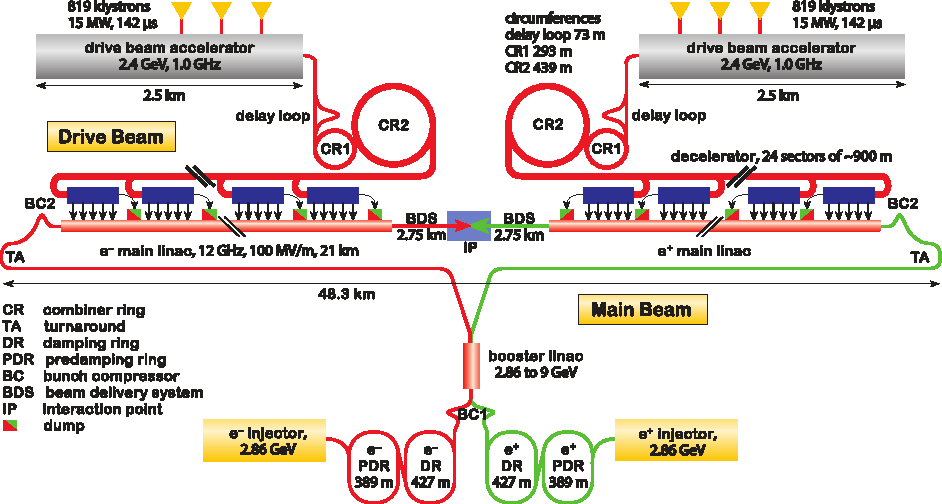
\includegraphics[width=\hsize]{Figures/introduction/clicLayout}
  \caption{Layout of the CLIC complex.}.
  \label{f:clicLayout}
\end{figure}
\end{landscape}}

Conventional klystrons cannot produce the short pulse lengths and high peak powers required for CLIC [REF]. To achieve the necessary specifications with klystrons RF pulse compressors would have to be used to increase their output power and decrease their pulse length by roughly a factor 5 [REF]. This would require a prohibitively large number of klystrons, approximately 35000, and yeild a low RF power efficiency of about 40\% [REF]. To solve this problem CLIC proposes to use a novel two beam acceleration concept, in which the high energy main beam is accelerated using RF power extracted from a secondary, high intensity but low energy, drive beam.

Figure~\ref{f:clicLayout} shows the layout of the CLIC complex. The bottom half of the figure shows the generation of the main colliding beams. The electron and positron beams are generated in dedicated injectors at the bottom of the figure, where they are accelerated to an energy of 2.86~GeV. They are then transported to a series of damping rings, in which the effects synchrotron radiation are used to decrease the beam size [REF]. After leaving the damping rings they are accelerated further to 9~GeV before being transported to each end of the main linac. Here both beams are accelerated in 21~km linacs containing the 100 MV/m accelerating structures, reaching an energy of 1.5~TeV. Finally, the beam size is squeezed further in the beam delivery system (BDS), down to the nanometre sizes necesarry to achieve high peak luminosity, before being brought in to collision at the interaction point.

The top half of the figure shows the beam lines involved in the generation of the high intensity drive beams. The drive beam accelerators are conventional linacs with an RF frequency of 1~GHz, a beam pulse length of 142~\(\mathrm{\mu s}\), a beam current of 4.2~A and a final energy of 2.4~GeV. The longer beam pulse length and lower power requirements means klystrons can be used with high efficiencies, unlike the main beams. Following the linac the drive beams enter a series of ``delay loops'' and ``combiner rings'' in which the drive beam is interleaved with itself to increase its intensity by a factor 24 (to 100~A) in a series of shorter 240~ns beam pulses. This drive beam recombination process is described in Section~\ref{ss:clicCombination}.

The 100~A drive beam is then directed in to 24 decelerator sections. Here a series of specially designed cavities, Power Extraction and Transfer Structures (PETS), are installed which decelerate, and extract power from, the drive beam. The PETS extract 90\% of the energy of the drive beam [REF], creating an RF pulse with the necessary properties to accelerate the main beam at 100~MV/m. The extracted RF power from the PETS is transferred to the main beam accelerating cavities via short waveguides.



\subsection{Drive Beam Recombination}
\label{ss:clicCombination}

The combination process used to produce the high intensity drive beam pulses is a unique feature of CLIC. The intensity is increased by a factor 2 in the delay loop, a factor three in the first combiner ring (CR1) and a factor 4 in the second combiner ring (CR2) to give the overall increase of \(2 \times 3 \times 4 = 24\) in beam current. 

\begin{figure}
  \centering
  \includegraphics[width=0.9\textwidth]{Figures/introduction/delayLoop}
  \caption{Drive beam recombination in the delay loop [REF].}.
  \label{f:delayLoop}
    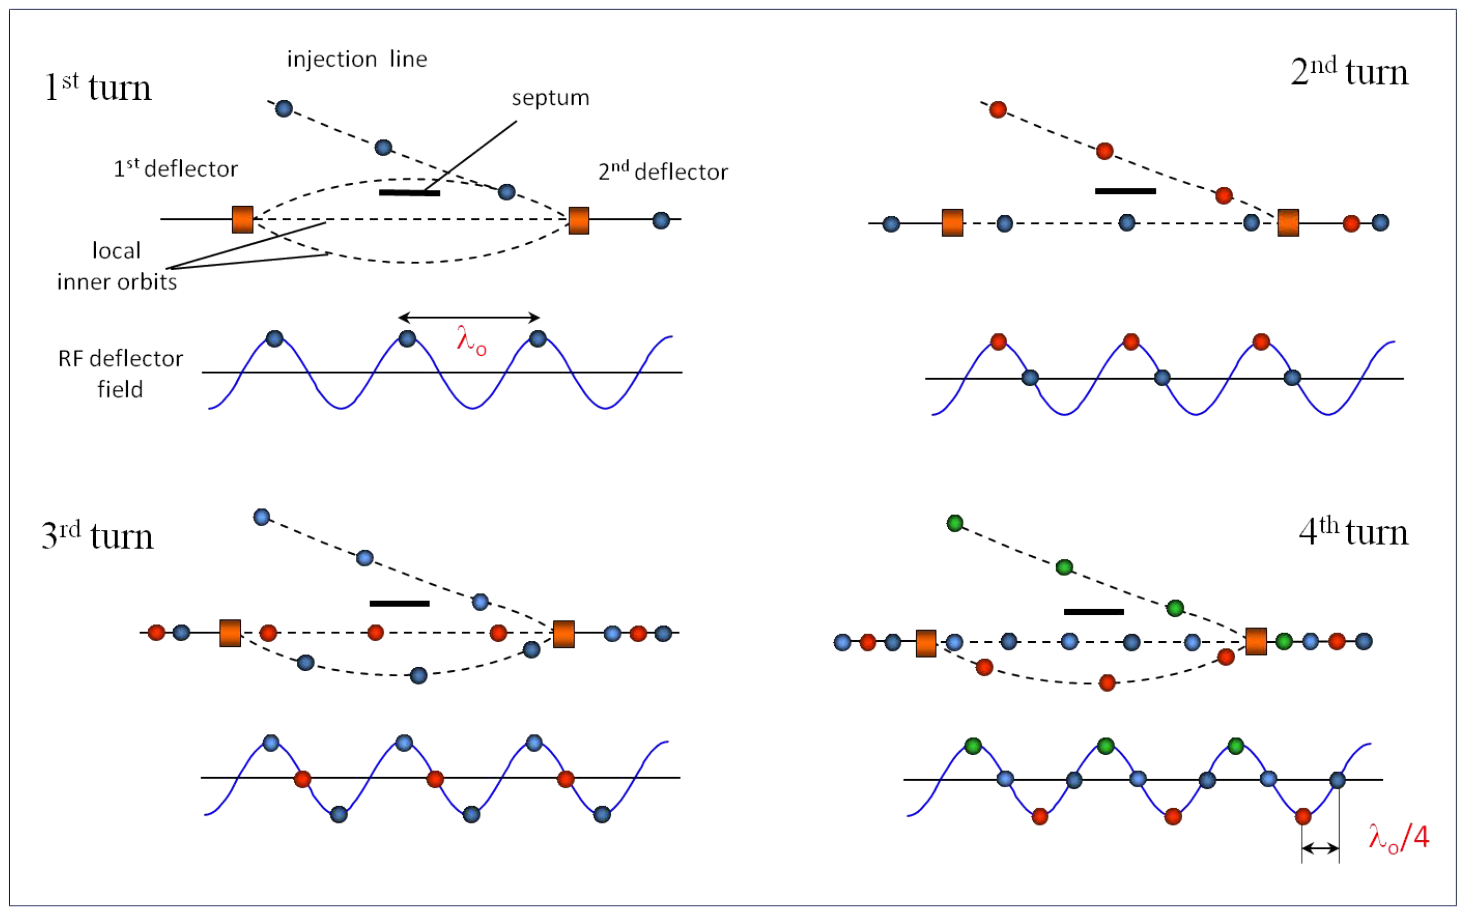
\includegraphics[width=0.9\textwidth]{Figures/introduction/combinerRing}
  \caption{Drive beam recombination in the second combiner ring [REF].}.
  \label{f:combinerRing}
\end{figure}

Figure~\ref{f:delayLoop} shows the recombination process in the delay loop. Although the drive beam acceleration frequency is 1~GHz it is bunched at 0.5~GHz. At 240~ns intervals along the \(142~\mathrm{\mu s}\) drive beam pulse the phase of the bunching is switched by \(180^\circ\) at 0.5~GHz. This phase switching is performed by sub-harmonic bunchers (SHBs) powered by travelling wave tubes (TWTs). As \(180^\circ\) at 0.5~GHz is a full \(360^\circ\) at the acceleration frequency of 1~GHz the phase switching has no effect on the acceleration of the drive beam. 

At the entrance of the delay loop a 0.5~GHz RF deflector is used. The 240~ns sub-trains alternate between having bunches that arrive when the field in the RF delfector is positive or negative. Sub-trains arriving when the field is positive are deflected in to the delay loop, whereas the remaining sub-trains bypass it. The length of the delay loop is also precisely tuned to be 240~ns, so that the sub-trains leaving the delay loop merge with the following sub-train bypassing the delay loop. The bunch frequency and beam current following the delay loop are therefore doubled to 1~GHz and 8.4~A respecitvely. The resulting beam structure consists of 240~ns pulses separated by 240~ns gaps.

A similar process takes place in the two combiner rings to give the final 12~GHz bunch frequency and 100~A beam current. Figure~\ref{f:combinerRing} shows the recombination of a factor 4 in CR2. RF deflectors are again used to inject the beam in to the ring, this time with a higher frequency 3~GHz deflecting field to match the bunch frequency of the drive beam following CR1. The first drive beam sub-train entering CR2 circulates the ring for four turns. The length of the ring is chosen so that the second sub-train arrives just as the first sub-train has completed one turn in the ring, with a delay of one quarter of the 3~GHz wave length. Repeating this for a further two turns, interleaving a new sub-train with the beam in the ring after each turn, yields the factor 4 increase in bunch frequency and therefore beam current. CR1 operates in the same way, but the beam circulates for three turns and the required path length difference is one third of the 1~GHz wavelength.

\newsection{clicPFF}{Phase Feedforward for CLIC}

phase jitter vs. luminosity

expected phase jitter plot

source of phase jitter

proposed layout of system to remove it - turnarounds before extraction. beat timing of beam etc.

required specifications - hardware power, bandwidth, latency etc.

\newsection{ctfIntro}{The CLIC Test Facility CTF3}

The CLIC design requires the use of many new concepts and technologies. Therefore, to prove the feasibility of CLIC the test facility CTF3 at CERN has been in operation since 2001 [REF]. It aims to demonstrate the generation of a high intensity drive beam using the bunch recombination process, as well as the extraction of power from this drive beam and the use of the extracted power to accelerate another beam. CTF3 also hosts many related activities in areas such as the development of 12~GHz accelerating cavities and beam instrumentation, for example [REF]. The main goals of CTF3 have been achieved and 2016 will be its last year of operation [REF].

A diagram of the CTF3 facility is found in Figure~\ref{f:ctfLayout},  showing the layout of buildings (purple) and beam lines (red) with the names and extent of the main sections labelled in black. The source of the CTF3 beam, at the top left of the figure in the linac, is a thermionic electron gun [REF] that produces a \(1.4~\mathrm{\mu s}\) beam pulse with an intensity of 4~A and a repetition rate of 0.8~Hz. The first 200~ns of the pulse contains a sharp energy transient and is eventually lost in the first bending sections of the facility, creating a usable pulse length of around \(1.2~\mathrm{\mu s}\). The continous beam pulse from the gun is bunched at either 1.5~GHz or 3~GHz depending on the mode of operation [REF].

\afterpage{\begin{landscape}
\begin{figure}
  \centering
  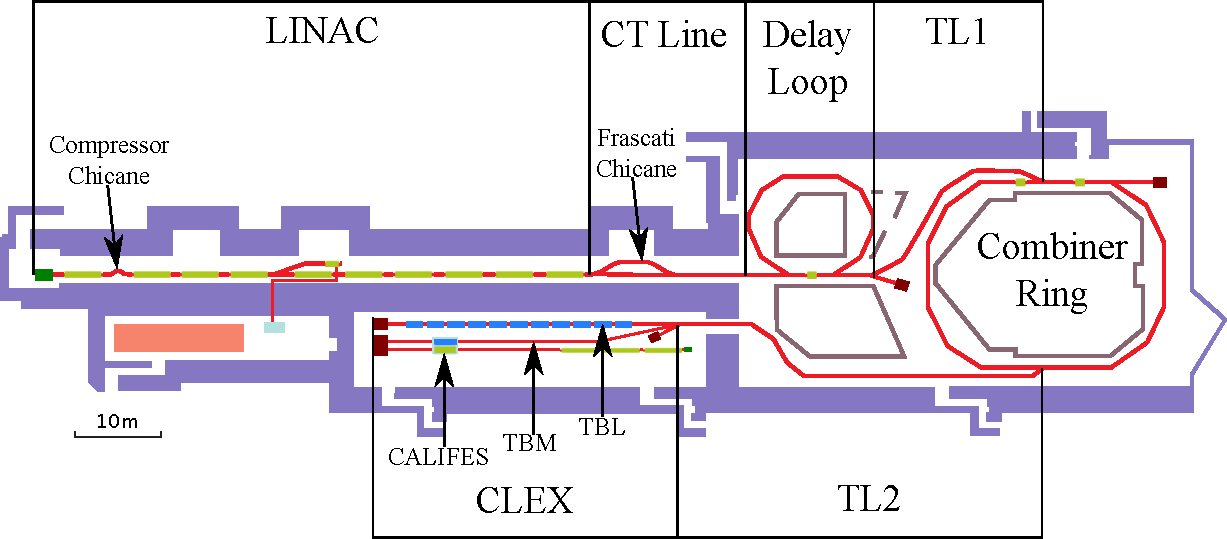
\includegraphics[width=\hsize]{Figures/introduction/ctfLayout}
  \caption{Layout of CTF3 with the main sections labelled.}
  \label{f:ctfLayout}
\end{figure}
\end{landscape}}

The beam is accelerated along the linac in 3~GHz RF cavities powered by conventional klystrons combined with RF pulse compressors which double their output power [REF]. The accelerating cavities are operated in the fully loaded mode, in which almost all the RF power sent to the cavity is absorbed by the beam for high power efficiency [REF]. At the end of the linac the beam reaches an energy of approximately 135~MeV.

Following the linac the beam intensity can be increased by up to a factor 8 using the delay loop and combiner ring, which both function in the same way as described for CLIC in Section~\ref{s:clicIntro}. Experiments at CTF3 are usually performed with either a 3~GHz factor 1 (4~A) or factor 4 (16~A) beam, or a 1.5~GHz factor 8 (28~A) beam. For the setups with 3~GHz bunching the delay loop is bypassed. The number of times the beam circulates around the combiner ring can be varied between 0.5 and 3.5 turns to give an increase in beam intensity by a factor 1, 2, 3 or 4. With 1.5~GHz beam a 1.5~GHz RF deflector [REF] is used at the delay loop entrance to inject alternating 140~ns sub-trains in to the loop. The sub-trains exiting the loop merge with the 140~ns trains bypassing the loop to give a factor 2 increase in beam intensity. The intensity of this factor 2 beam can then also be increased by additional factor 4 in the combiner ring, to give the total increase of a factor 8.

Following the combiner ring the beam enters the transfer line TL2, which transports the beam to the CLIC experimental area (CLEX). In CLEX the CTF3 drive beam can be directed to two different beam lines - TBL (Test Beam Line) and TBM (Two Beam Module). In TBL a series of PETS are installed to test the extraction of power from the drive beam and to measure the properties of the produced RF power [REF]. In TBM a prototype CLIC accelerating module is installed, in which RF power is extracted from the drive beam and used to accelerate a second beam, called CALIFES. The CALIFES beam also hosts many experiments independent from the CTF3 drive beam [REF].

\newsection{pffCTFIntro}{The PFF Prototype at CTF3}

The phase feedforward system proposed for CLIC (Section~\ref{s:}) presents many challenges in terms of the required hardware latencies, resolutions, power and bandwidth. As a result, one of the key activities at CTF3 since 2013 has been the design, installation and operation of a prototype PFF system. The primary goal of the PFF prototype is to demonstrate the feasibility of the PFF concept, with the ultimate aim of reducing the CTF3 phase jitter to close to the CLIC requirement of \(0.2^\circ\)~at~12~GHz, with a correction bandwidth above 17.5~MHz. The pursuit of this goal has required the development and installation of new hardware, as well as modifications and improvements to the setup and stability of the whole CTF3 drive beam complex.

The layout of the PFF prototype is shown in Figure~\ref{f:ctfpffLayout}. The overall concept is the same as the CLIC proposal -- the beam phase is measured prior to a turnaround and then corrected by changing the path length through a chicane using kickers. At CTF3 the PFF input is the phase measured in the CT line (\(\phi_1\) in the figure). The phase is then corrected using two kickers installed in the ``dog-leg'' shaped chicane in the TL2 transfer line.  A 3~GHz, uncombined beam is used, bypassing the delay loop (DL) and completing only half a turn in the combiner ring (CR). With this setup the time of flight between the phase monitor (\(\phi_1\)) and the first kicker (K1) is approximately 380~ns. Like the proposed CLIC system, the PFF prototype aims to apply the correction downstream (in TL2) to exactly the same pulse that was initially measured upstream (in the CT line), which is possible as the correction signals travel a shorter distance than the beam. The latency of the whole system, including the signal transit times in cables and hardware latencies, must therefore be less than 380~ns.

\afterpage{\begin{landscape}
\begin{figure}
  \centering
  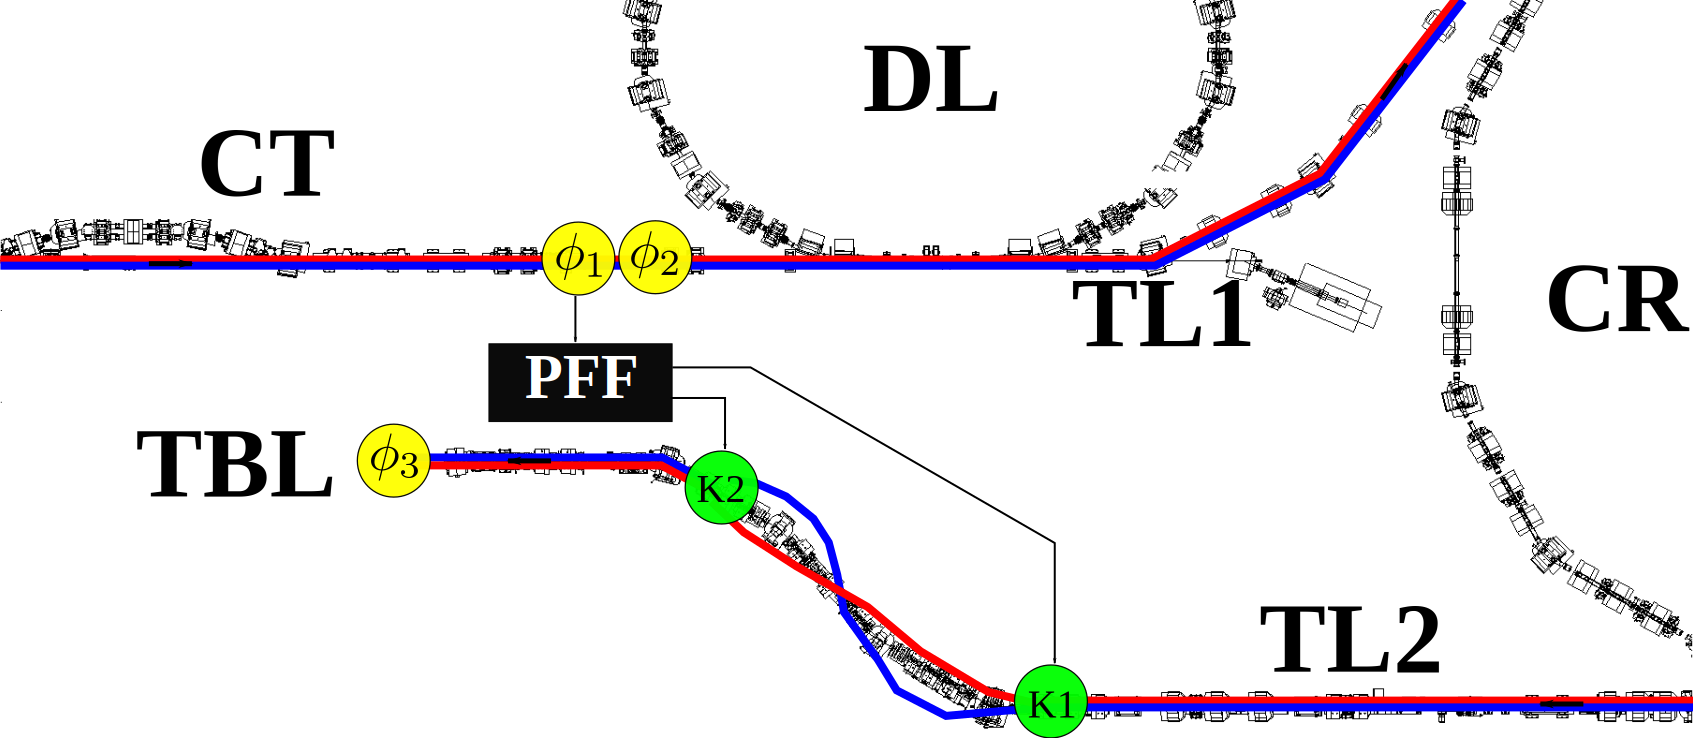
\includegraphics[width=\hsize]{Figures/introduction/ctfpffLayout}
  \caption{Schematic of the PFF prototype at CTF3, showing the approximate location of the phase monitors (\(\phi_1\), \(\phi_2\) and \(\phi_3\)) and the kickers (K1 and K2). The black box ``PFF'' represents the calculation and output of the correction, including the phase monitor electronics, feedforward controller and kicker amplifiers. A bunch arriving early at \(\phi_1\) is directed on to a longer path in the TL2 chicane using the kickers (blue trajectory), whereas a bunch arriving late will be directed on to a shorter  path (red trajectory)}.
  \label{f:ctfpffLayout}
\end{figure}
\end{landscape}}

\subsection{Hardware}
\label{ss:ctfPFFHardware}

The major hardware components of the PFF prototype are three phase monitors, two kickers, three sets of electronics for the phase monitors, a digitiser/feedforward controller and amplifiers to power the kickers (referred to as the kicker amplifiers). All the hardware components were designed, built and newly installed at CTF3 for the PFF prototype. The same components could be used at CLIC, with some important differences as described in Section~\ref{ss:ctfVsCLIC}. Each piece of hardware and its role is briefly introduced here, with more detail provided for each component in the remainder of the thesis.

The kickers and phase monitors are installed in the beam line at the locations shown in Figure~\ref{f:ctfpffLayout}, whereas the phase monitor electronics, feedforward controller and kicker amplifiers are installed in the CTF3 ``klystron gallery'', on the floor above the accelerator hall, for easier access. The cable lengths between the phase monitors and their electronics, and between the amplifiers and the kickers, are therefore longer than they appear in Figure~\ref{f:ctfpffLayout}.

As already described, the first phase monitor (\(\phi_1\)), in the CT line, provides the PFF input. The neighbouring second phase monitor (\(\phi_2\)), also in the CT line, is used to cross-check and verify the performance of the phase monitors. The final phase monitor (\(\phi_3\)), in the TBL line, measures the corrected phase jitter following the chicane in TL2. The phase monitors are designed by INFN, Italy [REF] to give a resolution below \(0.2^\circ\) at 12~GHz with a bandwidth above 30MHz, also taking in to account the  design of the phase monitor electronics [REF].

The processed signals from the first phase monitor are sent to the ``FONT5a board'', the feedforward controller designed and built by the Oxford University group of the John Adams Institute (JAI) [REF]. With a low latency of around 60~ns [REF], the FONT5a board digitises the phase monitor signals, calculates the appropriate correction to apply and provides the drive signal for the kicker amplifiers.

The kicker amplifiers have also been designed and built by Oxford University/JAI, and provide the voltage that produces the electric and magnetic fields that deflect the beam when applied to the kickers. Each amplifier module provides a power of around 20~kW with a bandwidth close to 50~MHz for small variations [REF]. 

Finally, the two kickers that provide the correction were designed and built by INFN, Italy. The are installed prior to the first and last dipoles in the TL2 dog-leg chicane, and deflect the CTF3 beam through an angle of 1~mrad for an applied voltage of around 1.3~kV [REF].


\subsection{Differences Between PFF at CTF3 and CLIC}
\label{ss:ctfVsCLIC}

The goal of the prototype is to prove the general PFF concept and the feasibility of using it to achieve \(0.2^\circ\) drive beam phase stability. It is neither necessary nor possible for the proposed CLIC and CTF3 systems to be identical, and there are a number of differences between the two that are summarised here. 

The most obvious difference between the applications at CTF3 and CLIC are the different beam energies and scale of the two complexes. CLIC will have a drive beam energy of 2.4~GeV, compared to the 135~MeV CTF3 drive beam. The CLIC PFF system therefore requires much higher power from the kicker amplifiers to deflect the beam by the same amount as the CTF3 prototype. CLIC requires up to 500~kW peak power from the amplifiers, compared to 20~kW at CTF3. Multiple amplifier modules with similar design to the CTF3 amplifiers could be combined to meet the CLIC power requirements [REF].

The CLIC proposal requires 48 separate PFF systems, with one in each of the 24 decelerator sections for each of the two drive beams. Aside from the vast difference in the quantity of required hardware components, the CLIC application also presents the challenge of synchronising the reference timing of the 48 systems along the 50~km facility with femtosecond stability. This is not adressed in the CTF3 prototype but feasible solutions have been proposed [REF].

Although both the CTF3 and CLIC schemes use chicanes to vary the beam trajectory the design of the chicanes used are different -- with a four bend C--shaped chicane with sixteen PFF kickers proposed in the CLIC CDR, compared to the four bend dog leg chicane at CTF3 with two PFF kickers installed for the correction. The freedom to design a purpose built chicane with additional kickers in the CLIC design somewhat simplifies the challenges of obtaining a suitable layout for the prototype chicane at CTF3 using pre-existing beam lines (Chapter~\ref{c:tl2Optics}).

Another key difference is that at CTF3 the PFF prototype is operated on uncombined beam, bypassing the delay loop and completing only half a turn in the combiner ring. At CLIC the complete PFF system (including the PFF input) is placed after the drive beam recombination, and therefore would operate on combined beam. At CTF3 as the PFF input is placed prior to the delay loop any attempt to operate the PFF prototype with combined beam would be complicated by having to use the measured uncombined beam pulse to correct the combined pulse following the combiner ring. Nevertheless, operation of the prototype with combined beam could be possible and may be attempted in future tests.

The main effect of using the uncombined pulse at CTF3 rather than the combined pulse as forseen for CLIC is that the beam pulse lengths are different. At CLIC \(0.2^\circ\) phase stability is needed across the 240~ns combined beam pulse. At CTF3 the uncombined pulse is much longer, up to 1.2~\(\mathrm{\mu s}\). It is therefore not necessary to demonstrate \(0.2^\circ\) phase stability across the full CTF3 pulse length to fulfill the CLIC requirements.

In fact, it is in any case impossible to demonstrate \(0.2^\circ\) phase stability across the full CTF3 pulse length with the PFF prototype due to the large phase sag that is present along the beam pulse. The RF pulse compression system at CTF3 [REF] results in an approximately parabolic variation of roughly \(40^\circ\) along the pulse which would not be present at CLIC. The phase sag is much larger than the correction range of the PFF prototype, which is designed to remove smaller, fast offsets. The PFF correction is therefore focused on the flatter, central part of the pulse around the minimum in the phase sag, where the phase variations across the pulse length relevant for CLIC are within the correction range. This is shown in Figure~\ref{f:ctfPhaseSag}.

\begin{figure}
  \centering
  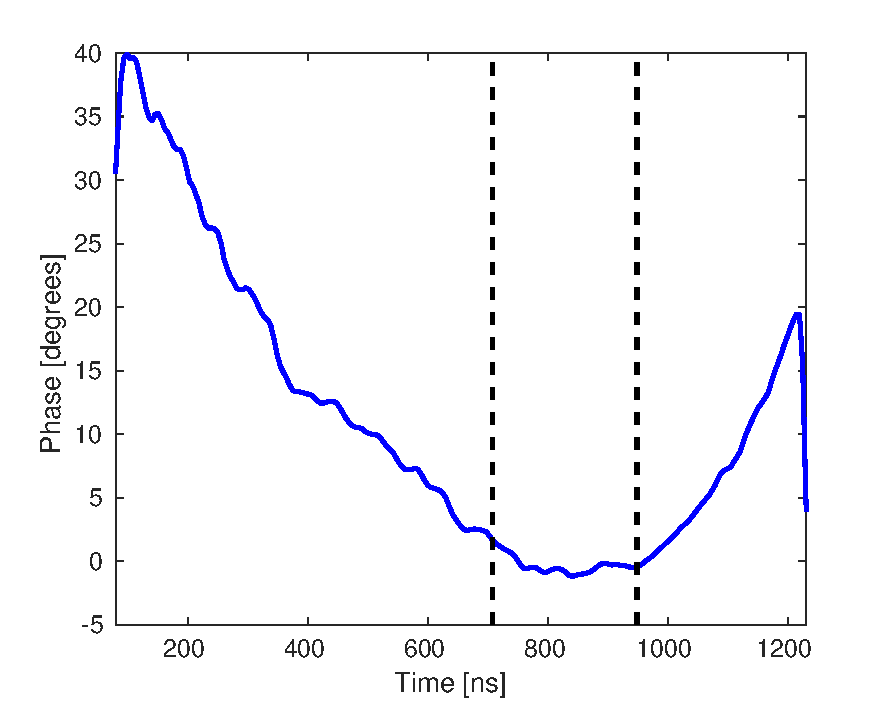
\includegraphics[width=0.8\textwidth]{Figures/introduction/phaseSag}
  \caption{Phase sag along the 1.2~\(\mathrm{\mu s}\) CTF3 beam pulse. The dashed black lines mark show the 240~ns combined CLIC pulse length centred around the region where the phase sag is flattest.}.
  \label{f:ctfPhaseSag}
\end{figure}

\newsection{phaseJitDefs}{Definitions of Different Phase Statistics}

Throughout the thesis several terms will be use to describe different ways of measuring the phase, as well as other parameters. These terms are briefly summarised here for reference. All quoted phase values throughout the thesis are in degrees at 12~GHz.

CTF3 provides an uncombined beam pulse length of up to 1.2~\(\mathrm{\mu s}\). It is useful to compare results both along the pulse and for the mean of the pulse. To calculate ``mean'' statistics, the average of each beam pulse is taken. Usually this is not taken across the full pulse length, but rather across a a region of several hundred nanoseconds near the mid-portion of the pulse where the beam is most stable and the phase sag is flattest. Mean statistics are usually plotted against time in units of the pulse number, with CTF3 operating at a repetition rate of 0.8~Hz, or one beam pulse every 1.25~s. The mean phase jitter represents the standard deviation of these mean values across the duration of a dataset.

Any statistic instead described as being ``along the pulse'' represents the measured values point by point along the beam pulse, typically sampled at a rate of a few hundred MHz. The time axes for plots of statistics along the pulse are either in units of nanoseconds, or simply the point number along the pulse (sample number). The phase jitter along the pulse represents the standard deviation of the measured phases at each individual sample point taken across the duration of a dataset.

Many of the discussions in the thesis also quote correlation coefficients, which in all cases are Pearson product-moment correlation coefficients [REF].

\newsection{thesisOverview}{Thesis Overview}

This thesis documents the design, commissioning, operation and results of the PFF prototype at CTF3. In Chapter~\ref{c:tl2Optics} the design of the TL2 chicane and the modifications to it that were necessary to achieve the desired phase shifting behaviour are described in more detail. 

The performance of the PFF correction depends on the ability to precisely measure the beam phase, and so Chapter~\ref{c:phaseMons} presents the extensive work that has been completed to understand and maximise the precision of the new purpose built phase monitors that were installed at CTF3 for the PFF system. 

As well as excellent precision in the measured phase, it is crucial to have high correlation between the phase at the end of the linac (the PFF input) and the phase at the correction location (TL2). With no correlation between the phases at these two points no improvement in phase jitter would be possible with the PFF system. Chapter~\ref{c:phasePropagation} describes the process of understanding and improving this correlation.

Chapter~\ref{c:commissioning} focuses on the setup of the remaining PFF hardware components and the commissioning of the complete PFF system. This includes the implementation of the PFF correction on the feedforward controller (the FONT5a board), the design and performance of the kicker amplifiers, as well as verifying the correction timing and correction range.

Chapter~\ref{c:feedforward} then presents the best results that have been achieved with the PFF prototype to date following all the optimisations described in the rest of the thesis. An analysis of the current limitations of the system and possible future improvements to the PFF setup are also discussed. Finally, the conclusions from each chapter and suggestions for future work are summarised in Chapter~\ref{c:conclusion}.

